\documentclass[a4paper,11pt]{article}
\usepackage{graphicx,url}
\usepackage{draftwatermark}
\SetWatermarkText{DRAFT}
\SetWatermarkScale{8}
%\usepackage[big,compact,sf]{titlesec}
%\usepackage{sidecap}
\usepackage{graphics,graphicx}
%\usepackage{verbatim}
%\usepackage{wrapfig}
%\usepackage{floatflt}
%\usepackage{times}
%\usepackage{multicol}
\usepackage{color}
\newcommand{\red}{\textcolor{red}}

%\usepackage{sober}
%\usepackage[small,compact,sf]{titlesec}

\newcounter{fred}

\newcommand{\mic}{\mu{\rm m}}
\def\es{\mathrel{\rm e^-/s}}
\def\pix{\mathrel{\rm pix}}
\def\elec{\mathrel{\rm e^-}}
\def\kpc{\mathrel{\rm kpc}}
\def\Gpc{\mathrel{\rm Gpc}}
\def\Msol{\mathrel{\rm M_{\odot}}}
\def\fsub{\mathrel{f_{\rm sub}}}
\def\Mtot{\mathrel{M_{\rm tot}}}
\def\ls{\mathrel{\hbox{\rlap{\hbox{\lower4pt\hbox{$\sim$}}}\hbox{$<$}}}}
\def\gs{\mathrel{\hbox{\rlap{\hbox{\lower4pt\hbox{$\sim$}}}\hbox{$>$}}}}
\def\Msolpyr{\mathrel{\rm M_{\odot}\,yr^{-1}}}
\def\mas{\mathrel{\rm mas}}
\def\pc{\mathrel{\rm pc}}
\def\Ho{\mathrel{H_{\rm 0}}}
\def\oM{\mathrel{\Omega_{\rm M}}}
\def\oL{\mathrel{\Omega_{\rm \Lambda}}}
\def\kms{\mathrel{\rm km\,s^{-1}}}
\def\ms{\mathrel{\rm m\,s^{-1}}}
\def\m{\mathrel{\rm m}}
\def\nm{\mathrel{\rm nm}}
\def\mm{\mathrel{\rm mm}}
\def\cm{\mathrel{\rm cm}}
\def\km{\mathrel{\rm km}}
\def\um{\mathrel{\mu{\rm m}}}
\def\ang{\mathrel{\rm \AA}}
\def\Mpc{\mathrel{\rm Mpc}}
\def\ksec{\mathrel{{\rm ksec}}}
\def\mag{\mathrel{\rm mag}}
\def\Gyr{\mathrel{\rm Gyr}}
\def\Hz{\mathrel{\rm Hz}}
\def\MHz{\mathrel{\rm MHz}}
\def\GHz{\mathrel{\rm GHz}}
\def\THz{\mathrel{\rm THz}}
\def\PHz{\mathrel{\rm PHz}}
\def\EHz{\mathrel{\rm EHz}}
\def\Js{\mathrel{\rm Js}}
\def\J{\mathrel{\rm J}}
\def\W{\mathrel{\rm W}}
\def\eVs{\mathrel{\rm eV\,s}}
\def\eV{\mathrel{\rm eV}}
\def\K{\mathrel{\rm K}}
\def\Jy{\mathrel{\rm Jy}}
\def\mJy{\mathrel{\rm mJy}}
\def\uJy{\mathrel{\rm \mu Jy}}
\def\sr{\mathrel{\rm sr}}
\def\rad{\mathrel{\rm rad}}
\def\deg{\mathrel{\rm deg}}
\def\degsq{\mathrel{\rm deg}^2}
\def\fwhm{\mathrel{\rm FWHM}}
\def\fried{\mathrel{r_0}}
\def\fo{\mathrel{f_{\rm o}}}
\def\fe{\mathrel{f_{\rm e}}}
\def\s{\mathrel{\rm s}}
\def\dol{\mathrel{D_{\rm OL}}}
\def\dos{\mathrel{D_{\rm OS}}}
\def\dls{\mathrel{D_{\rm LS}}}


\newcommand{\captionfonts}{\small}
\makeatletter  % Allow the use of @ in command names
\long\def\@makecaption#1#2{%
  \vskip\abovecaptionskip
  \sbox\@tempboxa{{\captionfonts #1: #2}}%
  \ifdim \wd\@tempboxa >\hsize
    {\captionfonts #1: #2\par}
  \else
    \hbox to\hsize{\hfil\box\@tempboxa\hfil}%
  \fi
  \vskip\belowcaptionskip}
\makeatother   % Cancel the effect of \makeatletter


\setlength{\textwidth}{172mm} 
\setlength{\textheight}{260mm}
\setlength{\topmargin}{-20mm} 
\setlength{\oddsidemargin}{-5mm}
\setlength{\evensidemargin}{10mm} 
\setlength{\headheight}{5mm}
\setlength{\headsep}{5mm} 
\setlength{\hoffset}{0in}
\setlength{\voffset}{0in}

\parskip=2truemm                       % Paragraph spacing
\parindent=4truemm                       % Paragraph indentation

\begin{document}

\pagestyle{myheadings}\markright{LSST:UK Galaxy Clusters White Paper 2016}

\sloppy

\pagestyle{empty}

~\vspace{70mm}

\centerline{\LARGE\bf LSST:UK Galaxy Clusters}
\bigskip\bigskip\bigskip
\centerline{\Large\bf High Level Science Interests and Science Requirements}
\medskip
\centerline{\Large\bf of the UK Galaxy Clusters Community}
\medskip
\centerline{\Large\bf as they relate to LSST}
\bigskip\bigskip\bigskip
\centerline{\Large\bf White Paper 2016}

\vspace{90mm}

\large
\noindent{\bf Last updated}: July 8, 2016

\noindent{\bf Contributors}: Malcolm Bremer, Chris Collins, Alastair
Edge, Nina Hatch, Ben Maughan, Graham Smith (coordinator), et al. {\it
  [add your name here]}


\newpage
\pagestyle{myheadings}
\setlength{\topmargin}{-10mm}
\setlength{\textheight}{255mm}

\tableofcontents

\newpage

\section{Introduction}\label{sec:intro}

{\it [Responsible: Graham Smith]}

\noindent
The purpose of this document is to summarise and communicate the UK
galaxy cluster community's interests as they relate to future
exploitation of LSST.  Section 2 describes our interests and the high
level requirements that they place on LSST data and combining data
from LSST with data from other upcoming facilities, including
\emph{Euclid} and \emph{e-ROSITA}.  Section 3 distils the common
themes from our varied interests to form the basis for discussion with
other communities within LSST (both UK-based, and internationally),
and colleagues leading the development of other facilities.

It is also envisaged that this document, and the discussions that it
stimulates, will help to shape requests for funding for galaxy cluster
science in the future.  The LSST:UK Phase B proposal to STFC's PPRP
will be a key opportunity to secure funding to support the development
of computer algorithms that the UK community will need in order to
delivering world-class galaxy cluster science with LSST.

The names attached to science interests in Section 2 is based on
participation/discussion at the inaugural LSST:UK Clusters meeting on
June 7, 2016, and the follow-up telecon on July 7, 2016.  However this
document is open for anyone in the UK to join and contribute to.  The
aim is to be succinct, so please try to stick to no more than one page
per science interest in Section 2.

Do we need to add a section that discusses how our interests,
requirements on the data, and strengths compare with those of the US
community?

\section{Science Interests}\label{sec:interests}

UK astronomers play leading roles in numerous international surveys
that study galaxy clusters, including: CARLA, DES, GEEC, GEEC2,
GoGREEN, LoCuSS, XCS, and XXL.  All of these surveys build towards
future exploitation of LSST and other surveys post-2020.  The relevant
surveys that will have synergies with LSST for cluster science include
\emph{Euclid}, \emph{e-ROSITA}, and fourth generation SZ surveys.

To give an overview of the UK's science interests relating to galaxy
clusters, we list some recent research results from the UK community
that are relevant to LSST-based science: \\\red{GPS: please can
  colleagues edit entries in this list that are relevant to them?}
\begin{itemize}
\item constraints on the nature of dark matter (Harvey et al.\ 2015,
  Sci, 347, 1462)
\item measurements of intracluster light at $z=1$ (Burke et al., 2012,
  MNRAS, 425, 2058)
\item systematic census of activity in brightest cluster galaxies
  (Green et al., arXiv:1606.01251)
\item cosmological hydrodynamical simulations that reproduce the
  observed properties of galaxy clusters and groups (McCarthy et al.,
  2016)
\item testing chameleon gravity with clusters from the XMM Cluster
  Survey (Wilcox et al., 2015, MNRAS, 452, 1171)
\item exploring the structure of cluster cores using Hubble Frontier
  Fields observations (Jauzac et al., 2015, MNRAS, 452, 1437; Jauzac
  et al.\ arXiv:1606.04527)
\item galaxy evolution in clusters and groups (Sean McGee, others)
\item discovery of protoclusters around high-z radio galaxies (Hatch
  et al., ...)
\item X-ray scaling relations of clusters (Giles et al.\ 2016, A\&A,
  592, 3)
\item weak-lensing calibration of the masses of galaxy groups and
  clusters (Smith et al., 2016, MNRAS, 456, L74; Okabe \& Smith,
  arXiv:1507.04493; Lieu et al.\ 2016, A\&A, 592, 4).
\end{itemize}
The following sections outline the science interests of the UK's
galaxy cluster community as they relate to LSST, and describe the high
level science requirements that our interests place on LSST data, and
the combination of LSST data with data from other surveys.

\subsection{Detection of galaxy clusters at $z<1.5$}\label{sec:clusdet}

{\it [Responsible: Kath Romer; Contributors: Malcolm Bremer]}

\noindent\red{GPS: I've pasted a ``stream of consciousness'' (his
  words) from Malcolm on this topic, below.  In the telecon we agreed
  for this to be edited in to a section on general cluster detection
  (meaning not just at $z\gs1$), with ``Nina's'' section changing to
  focus just on ``protoclusters''.  In the title of these two sections
  I've suggested to delimit them by redshift, above and below z=1.5,
  but I'm not sure this works.  This section needs input from Kath re
  what she is learning through XCS/DES, and she also volunteered to
  take responsibility for this section.}

\subsubsection*{Optical/near-infrared cluster detection}

\noindent LSST photometry will make possible detailed searches for,
and studies of, the galaxy populations of distant clusters and
protoclusters over huge volumes of the high redshift Universe. When
combined with other ground and space-based data sets, the LSST
photometry will allow characterisation of galaxy evolution within
environments that are the progenitors of the densest regions in
today's Universe and relate the variation in that evolution to the
detail of the environment that the galaxies inhabit. The character of
these studies can broadly be split into two redshift regimes - both
from the point of view of the evolution of the (proto) clusters and
also from the use of the LSST data.

The behaviour of the galaxy populations that we see in clusters today
(e.g. the red sequence, morphology-density relationship etc) seems to
be traceable to the growth and nature of virialised system at
$1<z<2$. Certainly for those systems with virialised masses above
$\sim 10^{14}$M$_\odot$ at $z\sim 1$, the red sequence is clearly in
place. By $z\sim 1.5$, 1.5 Gyr earlier, the evidence for strong red
sequences in similar systems is significantly weaker. The 2-2.5Gyr
period before $z\sim 1$ is likely to prove crucial in the build up of
the red sequence, and by extension the morphology-density relation
seen in today's clusters. The need to target a large and
well-specified sample of systems at these redshifts in order to
elucidate this growth is therefore clear.

The LSST data alone will be sufficient to identify system with strong
red sequences to $z\sim 1.2$, as has been done already with CFHTLS and
similar data sets. Beyond that redshift, and certainly at $z>1.5$,
near-IR photometry is additionally required in order to identify
systems with Balmer/4000\AA\ breaks and obtain sufficiently accurate
photometric redshifts in order to demonstrate clustering at a single
redshift. So in order to explore the birth and establishment of the
red sequence in clusters, a combination of LSST and near-IR data will
be required. The most obvious source for this over the kind of sky
area probed by LSST is Euclid imaging. VISTA will have limited impact
given the area of sky covered to useful depths before it is converted
to a spectroscopic telescope.  Spitzer/IRAC imaging of sufficient
depth to identify clusters to $z\sim 2$ is available for a few hundred
square degrees, so will be of some help in these regions.

As recent results have demonstrated that the morphology of red
sequence galaxies evolves for several Gyr after their stellar
populations become passive, the Euclid-derived morphologies will
provide invaluable for detailed studies. In order to identify the
non-red sequence galaxy population which becomes increasingly
important with increasing redshift, similar data will be required to
obtain reliable photometric redshifts - LSST data alone is
insufficient.

\subsubsection*{Cluster verification via detection of the ICM}

\red{GPS: is it possible to distill some requirements on a joint
  SZ/e-ROSITA/Euclid/LSST dataset from this section?  the sooner we
  can make progress on this the better, to progress discussions with
  e-ROSITA colleagues in particular.}

Note that optical/IR- selection of high redshift clusters (or cluster
candidates) does not identify the same population as those identified
in X-ray selected samples. Even systems that are richer (in terms of
potential cluster galaxies) than the typical X-ray selected systems
often show little or no significant X-ray emission. Certainly this
implies that at $z>1$ optically/IR-selected clusters and cluster
candidates have significant different properties in terms of
virialisation/dynamics/ICM than the X-ray selected systems, and in
some or many cases may not even be true clusters, but rather end-on
filaments or chance superpositions.

In order to test the reality and characterise the dynamical maturity
of clusters identified by LSST, their ICM needs to be probed in order
to estimate both their baryonic and total masses. This can be done
through X-ray and S-Z observations Consequently, large-area ICM
surveys will complement LSST observations and enable the most secure
halo identification.

Wide-area X-ray observations will come from eROSITA, which should
detect clusters with limiting masses of a few x $10^{14}$M$_\odot$ out
to $z\sim2$. Elucidating details of their X-ray emission beyond
luminosity, crude gas mass estimates and physical extent will likely
require follow-up with Chandra or XMM-Newton. As an alternative,
deeper - 40ksec - XMM exposures, either from the archive or from
potential contiguous surveys (eg the proposed deeper version of the
XXL survey covering one or two 25 deg$^2$ patches of the southern
sky), will provide samples of X-ray selected clusters to a lower mass
limit (by a factor of 2-5) than eROSITA out to $z\sim 2$.

The expected surface density of such systems is currently unclear, but
the existing XXL survey (slightly deeper than most of eROSITA)
identifies of order 0.5-1 system per square degree between $1<z<1.3$.
Given the rarity of the most massive sources at the highest redshifts,
the most distant eROSITA sources will represent the rarest most
massive and most evolved clusters at high redshift.  On the on hand,
their rarity and advanced evolutionary state makes them interesting,
but on the other, they will be very atypical of the typical cluster
population at these redshifts.

Of the various S-Z surveys of the southern sky ACTpol and SPTpol will
identify the lowest mass systems out to $z\sim 2$, with limits
potentially comparable to those of the X-ray observations noted
above. The selection function is different (selecting on integrated
pressure rather than the square of the gas density), so a comparison
of the SZ and X-ray properties of LSST-identified high redshift
clusters could be highly diagnostic of the growth and evolution of the
ICM at this critical phase of cluster evolution.

The predicted mass limits for the ICM surveys (both X-ray and S-Z) are
based on assumed scaling relations between ICM properties and mass
which are untested at high redshift. As it is expected that
significant energy input into the ICM from AGN will significantly
change these relationships above $z>1$, determining the ICM properties
of LSST- detected cluster will provide the leverage to explore how
this feedback affects these scaling relationship vary with redshift
and give clear insight into the underlying astrophysics that jointly
affects the evolution of clusters, their galaxy populations and an AGN
they host.

\subsection{Detection of protoclusters at $z>1.5$}\label{sec:proto}

{\it [Responsible: Nina Hatch; Contributors: Malcolm Bremer]}

\noindent\red{GPS: I have a note from the telecon that we will need
  different LSST/Euclid catalogues for different aspects of
  proto-cluster science, but I didn't write down more detail than
  that.  Please add these comments and detail either in to this
  section and/or a nice new bullet in Section 3?}

\noindent We will use the LSST survey and deep drilling fields to
search for distant ($z >1$) clusters and protoclusters to study the
formation of clusters and their member galaxies. Cluster and
protocluster detection algorithms will concentrate on searching for
galaxy overdensities in redshift space which exhibit strong
Balmer/4000\AA break features over large areas ($\sim$
10\,arcmin$^{-2}$). Based on recent studies (e.g. Chaing et al. 2014),
(proto)cluster detection will require photometric redshifts with at
least $\Delta z/ (1+z)\sim2.5$\% precision at $z>1$. This requires a
strong synergy between Euclid and LSST data as the Euclid Y, J and H
images are essential to span over the Balmer/4000\AA\ break for
$z>1.5$ galaxies.

The depth of the final LSST catalogues are sufficient to detect
significant numbers of red galaxies within each (proto)cluster at
redshifts up to $z\sim1.7$. Clusters and protoclusters up to
$z\sim2.5$ can be detected in the deep drilling fields using similar
algorithms, and these fields will produce cleaner cluster samples at
$z<1.7$ due to their lower photometric redshift uncertainty.

For protoclusters at $z>2.5$, the Balmer/$4000$\AA\ break shifts
beyond the wavelength range of LSST and Euclid. Furthermore, the red
sequences of such distant protoclusters are less prominent (perhaps
non-existent). We therefore must use the Lyman break feature of
galaxies to locate $z>2.5$ protoclusters.

To locate protoclusters the images must be deep enough to robustly
identify a galaxy overdensity across a few sq. arcmin. This requires
us to detect at least $\sim2$ LBGs per sq. arcmin. To achieve this the
filter redward of the Lyman break must reach depths of 26-27 mag (AB),
and the filter blueward of the break must reach 27-28 mag [but more
  detailed simulations are needed]. This means:\\
\noindent $\bullet$~$z\sim3$ U-band dropouts will only be detected to
sufficient depths in the deep drilling fields as the U-band in the
main field survey is too shallow. \\
\noindent $\bullet$ ~Dropouts in the g- and r-bands ($3.5<z<4.5$) will
be detected to sufficient depths to locate protoclusters in the main
survey. \\
\noindent $\bullet$ ~The surface density of i- and z-band dropouts
will be too low to robustly identify protoclusters in both main and
deep drilling fields. [Although this is subject to change as the
  depths of the deep fields are not certain at this stage]

In summary, combining the LSST and Euclid surveys allows us to search
for $1<z<1.7$ clusters and $3.5<z<4.5$ protoclusters across the main
survey using photometric redshifts and Lyman break dropout
techniques. The deep drilling fields allow us to search for $z>1.7$
(proto)clusters using photometric redshifts, and $z\sim3$
protoclusters using U-band dropouts. The main requirement for locating
distant clusters and protoclusters is a good synergy between Euclid
and LSST data products. We require accurate photometric catalogues
based on Euclid detection images. The deep drilling fields are very
important and infrared (3.6 and 4.5\,$\mu$m) coverage of these fields
is highly desirable.

In preparation for LSST data we should develop and test algorithms to
locate distant clusters and protoclusters. Realistic simulated light
cones would help test these algorithms. Such light comes need to be
sufficiently large to contain significant numbers of high redshift
clusters and protoclusters, and they would be most useful if the
luminosity function of galaxies (at LSST and Euclid wavelengths)
matched that of the local Universe and up to $z\sim4$.

\noindent\red{GPS: I've pasted the following text from Malcolm here,
  because it relates explicitly to proto-clusters.  Please homogenize
  with the rest of the text in this section.  (Malcolm tells me he
  won't be offended if none of this text is used.)}

At higher redshifts $z>2-2.5$, it is expected that essentially all the
progenitors of today's clusters will be in multiple low mass pieces,
rarely if ever dominated by a higher mass kernel to which other lower
mass systems accrete.  These systems will not be dominated by clear
red sequences and in these respects can be considered a different
phase to structure/cluster growth than the systems we observe at
$z<2$.  Moreover, while the lower redshift clusters/pro-clusters
require more than LSST data to identify, the earlier stages of cluster
evolution can potentially be studied using just LSST data as many of
the galaxies within these systems at $z>2.5$ will be Lyman Break
Galaxies (LBGs) that can be selected from LSST data alone.

These star forming objects typically have an intrinsically flat
($f_\nu \sim $~ constant) spectrum broken by a combination of the
intervening Ly$\alpha$ forest and the object's Lyman break.  So
candidate high redshift proto clusters can be identified as
overdensities of LBGs with similar colours/photometric redshifts on
arcminute scales, with the technique viable from $2.5<z<6$. Given that
the LBG selection alone does not necessarily allow highly accurate
photometric redshifts (colour and strength of break can be affected by
variable-strength Ly$\alpha$ emission and a range in the intrinsic
colour for the systems), confirmation of these candidates will require
a broader range of photometry, or more likely confirming spectroscopy.
Indeed, if the selection of objects from LSST is combined with an
ambitious programme of follow-up spectroscopy, these forming
proto-clusters can be placeed within the 3-D context of the developing
larger-scale-structure of the young Universe, thereby giving insight
into how the earl evolution of galaxies is affected by their early
environment.

Multi-band follow-up of LSST-identified proto-clusters will enable a
broader census of their galaxy populations as clearly significantly
dust-extincted or even passive galaxies will be missed by the LBG
selection but will surely exist within these structures.  These can be
identified through fitting SEDs into the near/mid IR using other data
sets to supplement the LSST data, being guided by the estimated
redshift for a given proto-cluster derived from the LBG
population. So, as with the $1<z<2$ cluster work, the higher redshift
studies will clearly benefit from the inclusion of similar
multi-wavelength ground and space-based data to supplement the LSST
data set.

Although the above may indicate that there is a gap in the redshift
range over which we can study the early evolution of clusters, the
range $2<z<2.5$ is straightforwardly covered by LSST data supplemented
by further near-IR data. This enables object selection either from the
simple BzK (gzK for LSST) technique, or more usefully from fitting
good-quality photometric models to well-sampled wide-band SEDs. So, in
combination with suitable other ground and spaced-based data sets we
can probe the growth and evolution of clusters and their galaxy
populations over an unprecedented range in redshift $z\sim 6$ to
$z\sim 1$ - essentially over the first $\sim5-6$ Gyr of their growth.

\subsection{Intracluster light and low surface brightness emission} \label{sec:lsb}

{\it [Responsible: Chris Collins]}

\noindent\red{GPS: In the telecon we discussed how this section needs
  to be homogenized with the section on BCGs.  Please can Chris do
  this?}

\noindent
Understanding the build up of stellar mass at the centres of galaxy
clusters is a key component to our understanding of galaxy
evolution. The centres of rich clusters are dominated by Brightest
Cluster Galaxies (BCG) which are the most luminous galaxies in the
universe emitting photospheric light. Observational studies have
consistently indicated that the masses of BCGs change by a factor no
larger than $30\%$ over the cosmic time out to a redshift $ z~1$, with
some results suggesting considerably less change (e.g. Collins et al.,
2009, Nature, 458, 603; Zhang, et al., 2016, ApJ, 816, 98). These
results are in themselves interesting as they challenge current model
predictions, particularly compared to semi-analytic simulations of
galaxy evolution. Furthermore model independent estimates of the
expected growth rates of BCGs from counts of satellite galaxies in the
cores of clusters, indicate that significant stellar mass is available
to grow the BCG based on dynamical friction timescale arguments. The
stellar mass in fact manifests itself not as BCG growth but as diffuse
and extended low surface brightness Intra Cluster Light (ICL) which
appears to grow rapidly since a redshift $z~1$ (Burke et al., 2015,
MNRAS, 449, 2353). Furthermore, the component ICL in nearby rich
clusters is large, and can it appears can even dominate the BCG
stellar mass. However there is no consensus on how the ICL grows with
cosmic time or even how the ICL fraction depends on cluster mass or
other parameters, with different conclusions in the literature largely
due to varying data quality.

Our interest in using LSST data is to quantify the ICL as a function
of cluster properties and redshift to at least $z~1.5$. The faint SB
limits of LSST stacked data will provide powerful comparisons with the
new generation high resolution galaxy simulations such as EAGLES which
can make predictions at LSST depths. In order to achieve this it is
important to optimise the sky background, flat fielding and PSF
correction techniques on large angular scales for low surface
brightness emission. Here it is worth noting that LSST will detect the
ICL in nearby clusters in the early exposures, involving detections
out to at least 1 degree in the case of Virgo. Existing survey data do
not provide sufficiently robust optimisation at low surface
brightness. Recent work using KiDSS (Kelvin et al., 2016, in
preparation) indicates that the ICL cannot satisfactorily be measured
using the current survey data release due to sky background estimation
techniques optimised for galaxies. Scattered light also adds a
systematic component to the measured extended intensities. Our own
work on deep VLT data with HAWK-I on the VLT in the near-IR J window
indicates that consistently deep surface brightness levels (defined as
recovering $80\%$ of the total flux and estimated using fake ICL
signals) can be obtained using a time averaged running median filter
to estimate sky and an appropriate random dither pattern. Similar
points concerning the PSF have also recently been made (Lombilla et
al., 2016, LSST Belgrade) concerning LSST measurements of the low
surface brightness thick disk components of edge-on galaxies. There is
therefore an urgent need to simulate the effects of LSST observing
techniques and the determination of the PSF on large angular scales to
extract the maximum information on the faint cosmic light from
ultra-deep LSST imaging at depths reaching $r \simeq 30-33$ per
arcsec$^{-2}$.

\subsection{Brightest cluster galaxies}

{\it [Responsible: Alastair Edge]}

\noindent\red{GPS: Here is a summary of feedback from the telecon: (1)
  this section needs to be homogenized with the section on ICL, (2)
  text on scientific requirements needs to be added -- for example,
  merged LSST/Euclid catalogues, deblending accuracy, technical issues
  re disentangling BCG and ICL?, (3) what timescale and level of
  variability in AGN require to be measured, and what implications
  does this have for detailed understanding of the psf? -- please
  discuss with Mark Birkinshaw who included work on AGN variability in
  the LSST:UK Phase A proposal.}

\noindent
The Brightest Cluster Galaxy (BCG) in a cluster is in most clusters
substantially brighter than all other cluster members (by 1--1.5~mag)
and found at the dynamical centre of the cluster at, or close to, the
X-ray peak (Sanderson et al. 2009). These galaxies represent the most
massive stellar systems known and their properties can be used to
constrain their formation history and how it relates to the evolution
of their host cluster.

Most BCGs are dominated by an old stellar population and share the
same colour-magnitude sequence with the other early type galaxies in
the cluster. However, there is a significant population of BCGs that
exhibit recent star formation and/or an AGN core (Crawford et
al. 1999).  This subset of ``active'' BCGs are predominately found in
the most X-ray luminous clusters (Green et al 2016) and have
associated optical line emission and cold molecular gas (Edge
2001). The properties of the intracluster gas surrounding the BCG
appear to be the dominant factor in triggering this activity
(Cavagnolo et al 2008) with a sharp threshold in central entropy
marking the point where $>$90\% of BCGs below show optical line
emission and $<$5\% of those above have lines.

Therefore, if it is possible to identify which BCGs are significantly
bluer expected from the observed colours of the cluster population, we
can very efficiently photometrically select these objects and compare
their radio, MIR and X-ray properties to the more passive BCGs. In the
radio the average power of a BCG which exhibits optical line emission
is an order of magnitude higher than that in non-line emitting systems
(Hogan et al. 2015).

The depth and coverage of LSST, when combined with NIR and MIR data
from Vista VHS and AllWISE, will be able to select these peculiar BCGs
in any cluster within $z\sim 1.0$ and the more extreme examples out to
$z>1.5$. The combination of multi-band photometry and multi-frequency
radio data will allow us to determine if the AGN and star-formation
activity in BCGs evolves significantly over the majority of the
lifetimes of all clusters.

In addition to the photometric properties of BCGs, LSST will also
provide important morphological information. For instance, N-body
simulations suggest that the majority of the growth of BCGs is through
the merger with other massive, early type galaxies (De Lucia \&
Bliazot 2007). Therefore a significant fraction of BCGs should have
the multiple nuclei expected for two galaxies in the latter stages of
these massive mergers. These systems are known but a significant
fraction may be chance alignments given the very high surface density
of galaxies in a cluster core. The quality and coverage of LSST will
provide the statistics to assess the probabilty of chance alignment
and the relative brightness of the components in a BCG to the likely
merger rate of BCGs can be determined as a function of redshift and
cluster mass.

The LSST imaging will also identify BCGs with extended stellar
envelopes, usually refered to as cD haloes, that extend on
$\approx$100~kpc scales blending into what can be defined as
Intracluster Light (see Chris's section?).  This extended halo is
often quite asymmetric and can contain shells and other evidence of
merger activity. Again, the depth and consistency of the LSST data
will allow us to determine the properties of these extended haloes
with other cluster properties over a wide range in redshift.

Finally, a small fraction of BCGs contain a sufficiently bright active
nucleus that variability can be detected. The most prominent example
of this is NGC1275 in the Perseus cluster (Kingman \& O'Connell et
al. 1979) which has shown two episodes of strong AGN activity in the
past 50 years (Dutson et al. 2014). The optical variability is
significant (0.2--0.4~mag on week to month timescales) so the LSST
sensitivity and cadence is very well matched to search for variability
from difference imaging and raw photometry. The fraction of BCGs
exhibiting strong, variable AGN will set important constraints on the
duty cycle of activity in BCGs and the accretion rate relative to the
Eddington limit during these AGN outbursts.  These factors are vital
to establish how AGN activity drives the vast amounts of energy out
into the surrounding intracluster gas through AGN feedback.

\subsection{Absolute mass calibration of galaxy clusters}\label{sec:mass}

{\it [Responsible: Graham Smith; Contributors: Ben Maughan]}

\noindent\red{GPS: In the telecon we discussed how this section needs
  to be generalised to discuss mass calibration for astrophysics as
  well as cosmology, especially for $z>1$ clusters (and protoclusters)
  because lensing won't help us at these redshifts.  This section
  needs to be coordinated with the new section on cluster physics.}

\noindent
Accurate absolute mass calibration of galaxy cluster samples out to
$z\simeq1$ and down to $M_{200}\sim5\times10^{13}M_\odot$ is essential
if clusters are to deliver a competitive constraint on dark energy.
This mass calibration will come from weak-lensing measurements using
optical survey data, because the basic measurements (galaxy shapes)
will be available directly from the optical survey data, and
weak-lensing probes directly the total mass distribution of clusters.
Recent progress on the mass calibration of clusters includes
measurements of massive clusters at $z<0.3$ with the lowest systematic
biases to date (Okabe \& Smith, 2016), and applying weak-lensing
techniques to poor clusters and rich groups (Lieu et al.\ 2016).

The most difficult systematic biases to control are those relating to
the selection of background galaxies, and then placing the background
galaxies accurately along the line of sight behind the clusters.  In
the LSST era the background galaxies will have apparent magnitudes of
${\rm AB}\sim23-27$, i.e.\ dominated by galaxies beyond the current
spectroscopic limit.  To obtain photometric redshifts with well
understood uncertainties, and to prove that the uncertainties are well
understood therefore requires deep spectroscopy way beyond the current
spectroscopic limit of ${\rm AB}\sim23-24$.  This is true even if we
accept that a useful level of spectroscopic completeness at the very
faintest limits is simply unachievable.

The challenge of controlling biases due to photometric selection and
photometric redshift estimation of background galaxies will be most
severe for high redshift clusters.  This is because the same optical
survey data of a given sensitivity will be used to select and
characterize the background galaxies for clusters independent of the
cluster redshifts.  Therefore higher redshift clusters are closer to
the background galaxies than the lower redshift clusters.
Consequently, the lensing kernel ($D_{\rm LS}/D_{\rm S}$; with which
the lensing signal scales linearly) is always a steeper function of
background galaxy redshift for higher redshift clusters than for lower
redshift clusters (Figure~1).

\noindent
\begin{minipage}{60mm}
%  \begin{figure}
    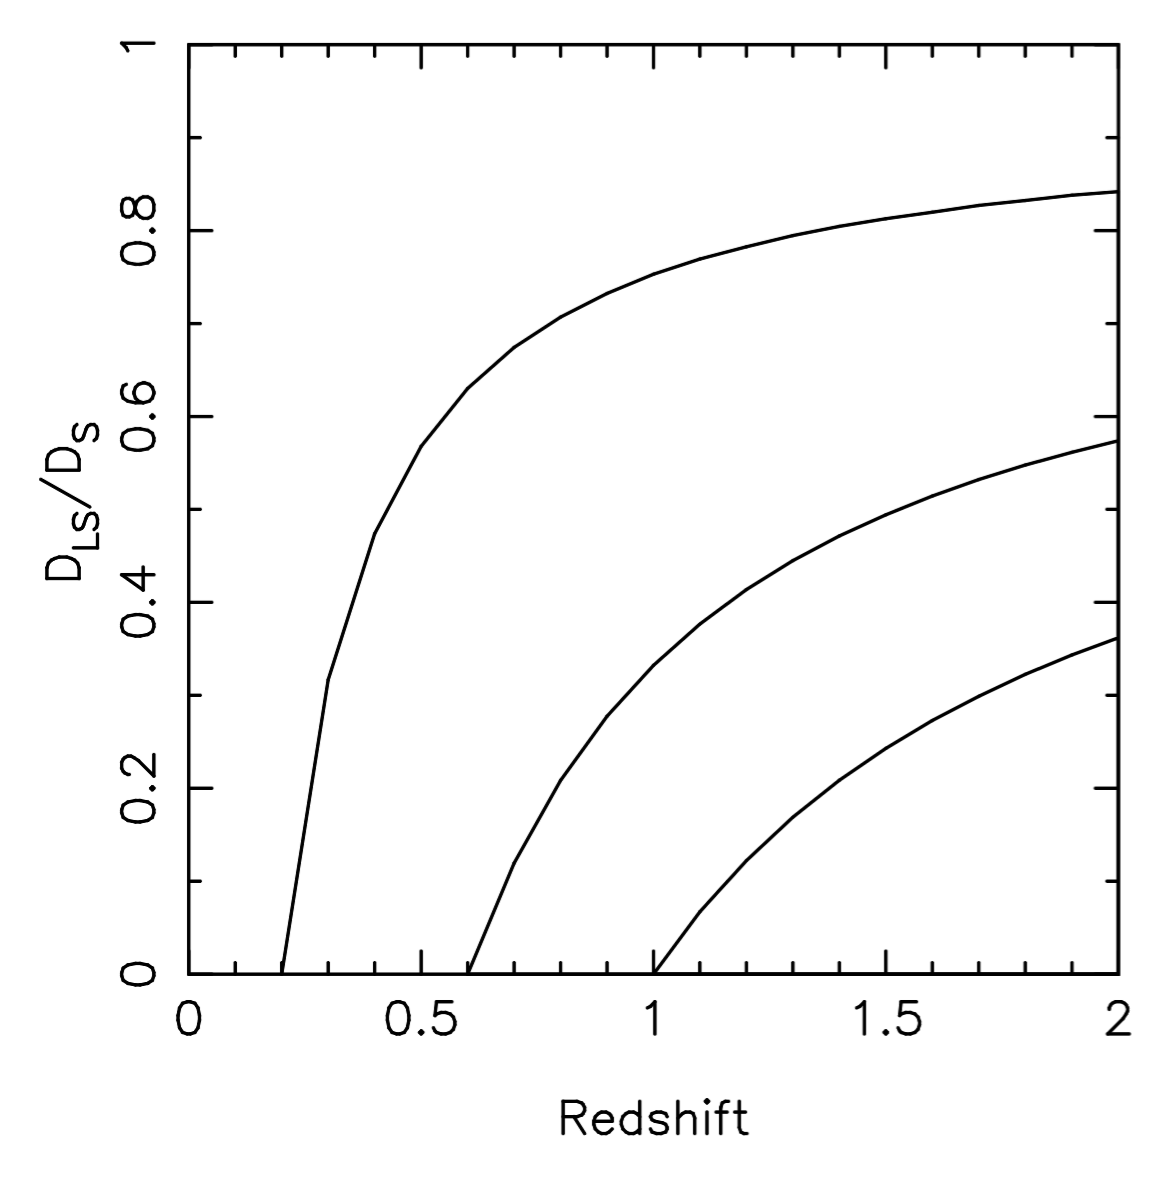
\includegraphics[width=\hsize]{dlsds.png}
\end{minipage}
\hspace{5mm}
\begin{minipage}{105mm}
  Figure~1: Dls/Ds ratio as a function of background galaxy redshift
  for cluster lenses at $z=0.2,0.6,1.0$. At any given background
  galaxy redshift the curve for the higher redshift clusters is
  steeper than the curve for lower redshift clusters.  Therefore the
  potential systematic bias due to mis-estimation of photometric
  redshifts is larger for higher redshift clusters.
\end{minipage}
%\end{figure*}

Building on the recent demonstration by Okabe \& Smith (2016) that
galaxies redder than the red sequence of cluster members in the
$(V-i)/i$ colour-magnitude plane offers a safe and calibratable method
to select galaxies behind massive galaxy clusters at $z\simeq0.2$, it
is important to explore how these methods can be extended to higher
redshifts.  Assuming for now that the rest-frame equivalents of $V$
and $i$-bands are the optimal filters for a red galaxy selection,
would motivate consideration of the $(i-J)$ colours for selection of
galaxies behind clusters at $z\simeq1$.  It is therefore clear that
photometry from \emph{Euclid} has an important role to play in
LSST-based cluster weak-lensing studies.  This point is further
amplified by the fact that merged LSST and \emph{Euclid} photometric
catalogues will be important for a broad range of extragalactic
science.  Given that this merged catalogue will be used to select
weakly-lensed background galaxies for which accurate shape
measurements are available, it is essential that the joint
LSST/\emph{Euclid} photometric catalogue production is based on the
same source identification as that used for the galaxy shape
measurement.  This begs the question of whether the source
identification for merged LSST/\emph{Euclid} photometric catalogues
should come from LSST or \emph{Euclid}?

Strategies that can be explored to improve/verify the accuracy of
photometric redshift estimates for galaxy cluster science include
choice of number, depth, and sky location of the deep drilling fields,
ultra-deep spectroscopic surveys of the deep drilling fields,
exploring how the \emph{Euclid} grism spectroscopy can assist with
spectroscopic calibration of photometric redshifts, development of
algorithms that include optical/X-ray/SZ information about the
over-densities along the line of sight through candidate clusters.

Galaxy clusters represent crowded lines of sight through the universe.
As such the requirements on the accuracy of deblended photometry are
more demanding than for typical lines of sight.  It is therefore
important to test the deblending capabilities of the LSST Data
Management team's software stack (DM Stack) on known clusters down to
$\sim5\times10^{13}M_\odot$ and out to $z\simeq1$.  It would be
sensible to do these tests on the most LSST-like data available today,
for example data obtained with Subaru telescope on massive low
redshift clusters, and also Hyper-Suprime-CAM (HSC) survey data.  On
this latter point, HSC has observed the XXL-N field to full survey
depth already.  This field contains clusters across the required
redshift and mass range.  The UK is well-placed to lead in this area
given the leading roles that we play in LoCuSS and XXL.  

\red{GPS: I've pasted here a couple of paragraphs from Ben that can
  help to improve this section, however some might end up in the
  cluster physics section..}

LSST will enable a diversity of mass measurements that can be tested
and cross calibrated to yield the precision and control of systematics
needed for cluster cosmology. Weak lensing masses from LSST will
anchor the calibration of mass proxies based on LSST photometry and
also those from complementary ICM surveys (both in X-rays and the SZ
effect). In the new LSST discovery space of high-z clusters and galaxy
groups at intermediate redshifts, stacking of the lensing, optical and
ICM-based mass proxies will be tested and calibrated. Discrepancies in
these regimes will yield new astrophysical insights. For example,
evolution or mass dependency of the baryon fractions, galaxy
demographics and ICM thermodynamic structure will all leave their
traces on the respective mass proxies.

Cluster cosmology is not the only motivation for reliable cluster mass
determinations. The mass is the single defining property of cluster
halos, providing the link between observation and simulations and the
context in which to set studies of galaxy and ICM evolution. For these
purposes, the requirements on mass precision are less demanding than
for cosmological studies. LSST and complementary surveys will enable
the investigation of these astrophysical processes at the very
frontiers of the observable mass and redshift space where the leverage
and discovery potential are the highest.

\subsection{Cluster physics}\label{sec:physics}

{\it [Responsible: Ben Maughan; Contributors: Graham Smith]}

\noindent\red{GPS: In the telecon we discussed adding this section,
  that will be about scaling relations, with Ben to write it (I'm
  happy to help).  So it will contain a fair bit of LSST/e-ROSITA
  synergy.  It would be very helpful to be as specific about that
  synergy as possible, because currently we're a lot more specific on
  LSST/Euclid synergy.  We also agreed to follow the DESC Clusters
  terminology of ``absolute mass calibration'' for WL-based mass
  measurements, and ``relative mass calibration'' for scaling relation
  studies.}

\subsection{Numerical simulations}\label{sec:sims}

{\it [Responsible: Ian McCarthy]}

\noindent\red{GPS: We didn't discuss simulations much in the telecon,
  although there was general agreement that we should try to generate
  a list of ``requirements on simulations'' ... in other words what do
  we need from simulations to support analysis of LSST data?  It's
  still not clear to me where to put a section on simulations in this
  document, given that it has a different nature to the other
  subsections in section 2 -- comments welcome.}

\section{Topics to discuss with the wider LSST community}

\red{GPS: Please can people have a go at writing bullets in this
  list?}

\noindent This is a preliminary list of galaxy cluster science
requirements to discuss with LSST colleagues:
\begin{itemize}
\item\underline{Low surface brightness emission
  (\S\ref{sec:lsb})}\smallskip\\Key questions: Will the currently
  envisaged observing strategy, standard data reduction pipeline, and
  steps to mitigate scattered light at the telescope conserve low
  surface brightness emission on degree scales in the single visit
  fits frames and the stacked multiple-visit fits frames?  Tests are
  required to examine impact of LSST observing strategy, data
  reduction pipeline, and scattered light on ability to recover faint
  low surface brightness emission from ourskirts of local galaxies
  (e.g.\ in Virgo), thick disk of edge-on galaxies, and intracluster
  light.  Key aspects of tests include the approach to flat-fielding
  and sky subtraction.  Tests on simulated data and on existing
  LSST-like data that would both be instructive.  
\item\underline{Merged LSST and \emph{Euclid} photometry and shape
  catalogues
  (\S\S\ref{sec:proto},\ref{sec:clusdet},\ref{sec:mass})}\smallskip\\kjskajk
  kjdksj dks dks jdk
\item\underline{Something about eROSITA synergy? (\S\S
  XX)}\smallskip\\ksjdksjd ksj dksj dk
\item
\item
\end{itemize}

%\subsection{Combining LSST and Euclid data products}

%\subsection{Combining LSST data with the e-ROSITA cluster catalogues}

%\subsection{Requirements on numerical simulations}

%\subsection{Requirements on data quality including flat-fielding}

%\subsection{Synergies with other Working Groups and Science Collaborations}

%\subsubsection{Weak-lensing}

%\subsubsection{Strong-lensing}

%\subsubsection{Galaxies}

%\subsubsection{Others?}

%\section{Summary}

\newpage

\appendix

\section{Glossary of acronyms including survey names}

\begin{itemize}
\item DESC -- Dark Energy Science Collaboration
\item GSC -- Galaxies Science Collaboration
\item DM -- Data Management team
\item ...
\item CARLA
\item GEEC and GEEC2
\item GoGREEN
\item LoCuSS -- Local Cluster Substructure Survey
\item XCS -- XMM Cluster Survey
\item XXL -- Ultimate Extragalactic XMM-Newton Survey
\end{itemize}

\section{UK leadership positions in international galaxy cluster surveys}

\begin{itemize}
\item
\item
\end{itemize}

\end{document}
